\documentclass[11pt,a4paper]{article}
\usepackage[utf8]{inputenc}
\usepackage[portuguese]{babel}
\usepackage[T1]{fontenc}
\usepackage{amsmath}
\usepackage{natbib}
\usepackage[pdftex]{color,graphicx}
\usepackage{setspace}
\setlength{\parindent}{0pt}
\usepackage{multirow}
\usepackage{amsfonts}
\usepackage{amssymb}
\usepackage{graphicx}
\usepackage[left=1.7cm,right=1.5cm,top=2.5cm,bottom=2cm]{geometry}
\usepackage{hyperref}
\usepackage{enumitem}  
\usepackage{subfigure}
\usepackage{float}


\renewcommand{\baselinestretch}{1.5}	



\pagestyle{empty}

\begin{document}


\begin{center}
\Large{\textbf{Um estudo sobre o desenvolvimento do nordeste }}

\bigskip

\begin{singlespace}
\large{Carolina Martins Crispim (UFF)

Daniel dos Santos (UFF)

Fernanda Fernandes (UFF)

Gabriel Mizuno (UFF)} 

\bigskip

\small{Github para consulta: \url{https://github.com/Daniel-EST/EST_aplicada}}
\end{singlespace}
\end{center}


\textbf{Resumo:} Este trabalho se propõe a criar um indicador composto que avalia o desenvolvimento humano nos municípios da região Nordeste do Brasil. O software utilizado para a manipulção e análise dos dados foi o R e Rstudio.


\textbf{Palavras-chave:} Nordeste, indicador, municípios, IDHM, R


\textbf{Introdução}

Com cerca de 56 560 081 habitantes. 2015 (wiki) e 9 estados com 1794 municípios a região nordeste possui um
A princípio reunimos indicadores dos municípios do Nordeste nos anos de 2000 e 2010, verificamos a correlação entre eles com a finalidade de criar um indicador composto para desenvolvimento humano, e então, validá-lo comparando-o com o IDHM. 


\textbf{Material e métodos}

Os dados procederam do site Atlas Brasil (\cite{atlas}) onde observamos os indicadores desejados nos anos de 2000 e 2010, sobre renda, educação e saúde dos municípios da região Nordeste. Com os indicadores em mãos organizamos a base de dados e em seguida padronizamos todas as variáveis usando a seguinte fórmula: $$\frac{V_{max}-V_{observado}}{V_{max} - V_{min}} $$ Em seguida, colocamos todas as variáveis no mesmo sentido, de forma que, quanto mais baixo o valor depois de padronizado melhor será para a população i.e. mortalidade infantil e taxa de analfabetismo. Aplicamos a Correlação de Pearson e consideramos que havia relação entre os indicadores com no mínimo 0.43 (mizuneca põe a tabela aqui). Sendo assim pegamos os seguintes indicadores Esperança de Vida ao Nascer, Mortalidade Infantil,  \% de Pobres, \% de Vulneráveis à Pobreza, Taxa de Analfabetismo e usamos da seguinte formula: $$ IC = \frac{EVN+MI+TA+P+VP}{5} $$ e então, validamos nosso indicador com o IDHM do mesmo site cuja fórmula é: $$ \sqrt[3]{\hbox{EDUCAÇÃO x LOGEVIDADE x RENDA}}$$ Geramos um gráfico de dispersão para uma análise descritiva da relação entre o Indicador Composto e o IDHM. E por último, confeccionamos um mapa temático com o nosso indicador composto por município. (faz referência mizuno!)


Devido a problemas na obtenção da base do site \cite{atlas} adotamos o seguinte critério para inputar sobre os dados faltantes:
\begin{enumerate}[label=(\roman*)]
\item fizemos uma média com os municípios que pertenciam a mesma microrregião. 
\item caso tenha apenas um munícipio na microrregião utilizamos um mapa para localizar os municípios mais próximos
\end{enumerate}

\textbf{Resultados e discussão}

Tendo em vista os resultados apresentados, como podemos notar (mizuno faz referência a tabela ou gráfico) as cores do mapa por município escureceram de 2000 para 2010, o que significa que o Indicador Composto aumentou, sendo assim o desenvolvimento piorou. Entretanto, quando usamos o IDHM para avaliar o desenvolvimento dessa região nos deparamos com uma leve melhora no mesmo período.

\begin{table}[h!]
  \begin{center}
      \caption{Tabela com algumas medidas resumo dos indicadores de 2000}
    \begin{tabular}{c|c|c|c|c|c|c|c}
    \hline
      \textbf{Indicador Composto} & \textbf{Min} & \textbf{1º Q} & \textbf{2º Q} & \textbf{Média} & \textbf{3º Q} & \textbf{Máx}  & \textbf{Desvio Padrão} \\
      \hline
      Esperança de vida & 57,46 & 56,48 & 63,88 & 64,16 & 65,92 & 74,75 & 2,56\\
      Taxa de Analfabetimos & 6,28 & 30,71 & 36,08 & 35,76 & 41,06 & 59,83 & 8,139\\
      \% de pobres & 0,98 & 58,42 & 65,80 & 64,47 & 72,11 & 89,99 & 10,95\\ 
      \% de vuneraveis a probeza & 7,19 & 80,67 & 85,23 & 83,89 & 88,79 & 99,00 & 7,49 \\ 
      Mortalidade & 21,4 & 42,52 & 48,62 & 49,09 & 54,65 & 96,37 &  9,736\\ 
      IDHM & 0,208 & 0,3820 & 0,4200 & 0,4222 & 0,6587 & 0,6840 & 0,0625 \\
      \hline
    \end{tabular}
     \label{table:1}
  \end{center}
\end{table}

\begin{table}[h!]
  \begin{center}
      \caption{Tabela com algumas medidas resumo dos indicadores de 2010}
    \begin{tabular}{c|c|c|c|c|c|c|c}
    \hline
      \textbf{Indicador Composto} & \textbf{Min} & \textbf{1º Q} & \textbf{2º Q} & \textbf{Média} & \textbf{3º Q} & \textbf{Máx}  & \textbf{Desvio Padrão} \\
      \hline
      Esperança de vida & 65,3 & 69,05 & 70,44 & 70,25 & 71,49 & 75,36 & 1,809 \\
      Taxa de Analfabetimos & 3,97 & 23,28 & 27,7 & 27,29 & 31,84 & 44,4 & 6,669\\
      \% de pobres & 2,2 & 34,61 & 41,95 & 41,51 & 48,72 & 78,23 & 10,89  \\ 
      \% de vuneraveis a probeza & 5,12 & 62,11 & 67,98 & 66,93 & 73,11 & 91,57 & 9,539 \\ 
      Mortalidade & 13,4 & 23,00 & 26,3 & 27,19 & 30,7 & 46,8 & 5,85\\ 
      IDHM & 0,443 & ,5623 & 0,588 & 0,5907 & 0,6140 & 0,7880 & 0,0432\\ 
      \hline
    \end{tabular}
     \label{table:2}
  \end{center}
\end{table}

\begin{table}[h!]
  \begin{center}
      \caption{Tabela com algumas medidas resumo do Indicador composto de 2000 e 2010}
    \begin{tabular}{c|c|c|c|c|c|c|c}
    \hline
      \textbf{Indicador Composto} & \textbf{Min} & \textbf{1º Q} & \textbf{2º Q} & \textbf{Média} & \textbf{3º Q} & \textbf{Máx}  & \textbf{Desvio Padrão} \\
      \hline
	  2000 & 0,1205 & 0,3131 & 0,3738 & 0,3838 & 0,4405 & 0,9978 & 0,104\\
	  2010 & 0,056 & 0,3754 & 0,44966 & 0,45419 & 0,52393 & 0,9948 & 0,1275\\
      \hline
    \end{tabular}
     \label{table:3}
  \end{center}
\end{table}


\begin{figure}[H]
\centering
\subfigure[Indicador Composto 2000]{ \label{subfig:IC2000}
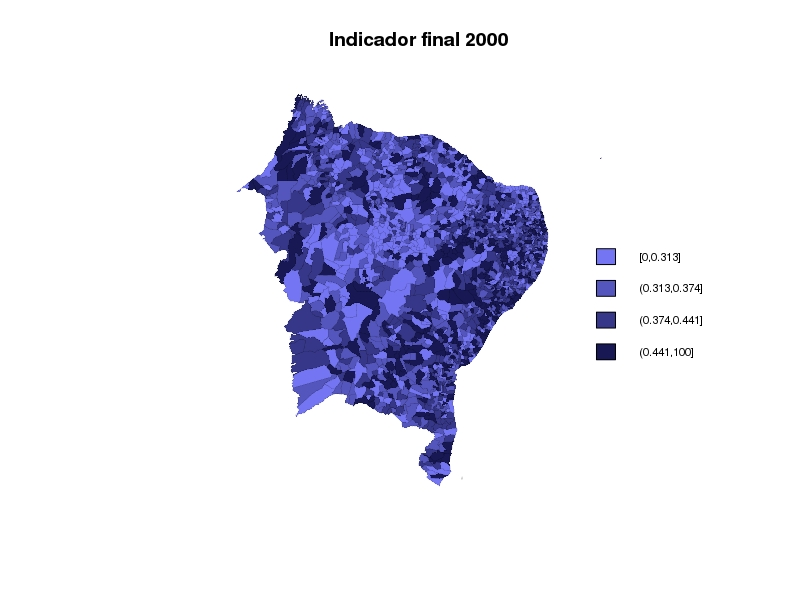
\includegraphics[width=0.4\textwidth]{Indicador_2000.jpg}
}\ \ \ \
\subfigure[Indicador Composto 2010]{            \label{subfig:IC2010}
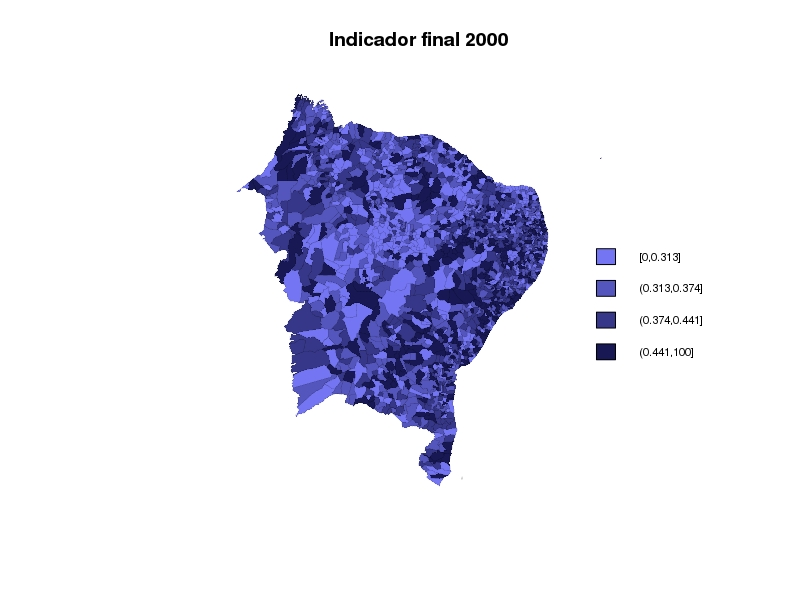
\includegraphics[width=0.4\textwidth]{Indicador_2000.jpg}
}
\caption{Mapas do Indicador Composto em 2000 e 20010.}
\label{fig:leao_grafico}
\end{figure}

\begin{figure}[H]
\centering
\subfigure[Indicador Composto 2000]{ \label{subfig:D2000}
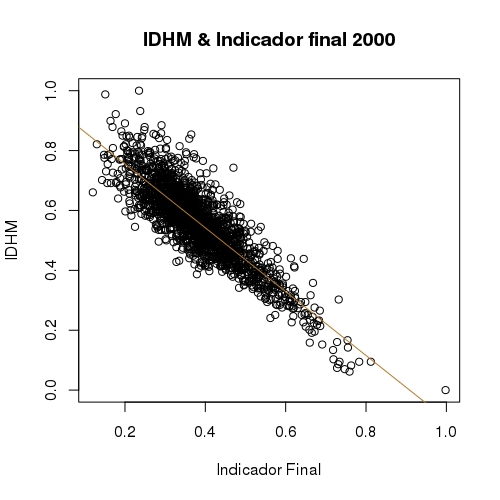
\includegraphics[width=0.4\textwidth]{Dispersao_2000.jpg}
}   \ \
\subfigure[Indicador Composto 2010]{            \label{subfig:D2000}
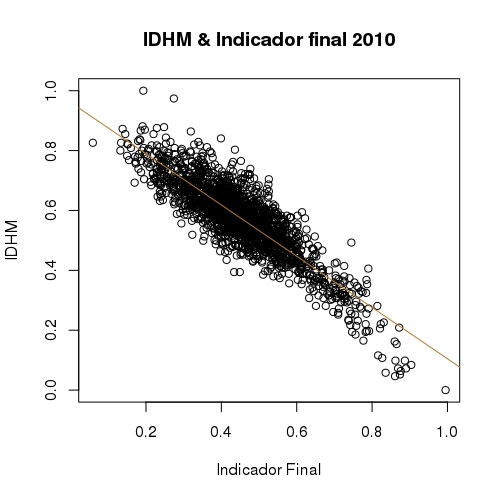
\includegraphics[width=0.4\textwidth]{Dispersao_2010.jpg
}
\caption{Figuras            apresentadas            com            o            pacote            \textit{subfigure}.}
\label{fig:D2010}
\end{figure}


\renewcommand{\bibname}{Referências}
\bibliographystyle{rss_port}
\bibliography{biblio}



%\renewcommand{\bibname}{"Bibliografia"}
%\bibliographystyle{plain}
%\bibliography{ref}

\end{document}